\chapter{Entwurfsklassendiagramm}
In diesem Kapitel wird das Entwurfsklassendiagramm erläutert. Es basiert im Wesentlichen auf dem Analyseklassendiagramm, allerdings wurden zusätzlich zu den im Analyseklassendiagramm identifizierten Klassen noch weitere für die Umsetzung nötige Elemente eingeführt und eine Einteilung in Pakete vorgenommen. Im Sinne der Übersichtlichkeit wurden im Entwurfsklassendiagramm statt der einzelnen Klassen die Packages eingefärbt. Lediglich die Klassen, welche persistiert werden sollen und darum das Interface \enquote{IPersistable} implementieren, wurden gelb eingefärbt. Es wird zunächst das Paket \enquote{model} beschrieben bzw. dessen Unterpakete, welche die Klassen aus dem Analyseklassendiagramm enthalten, gefolgt von den Packages der mit dem Entwurfsklassendiagramm eingeführten Klassen. Abschließend werden die im Entwurfsklassendiagramm verwendeten Entwurfsmuster beschrieben.
\FloatBarrier
\begin{figure}[ht!]
    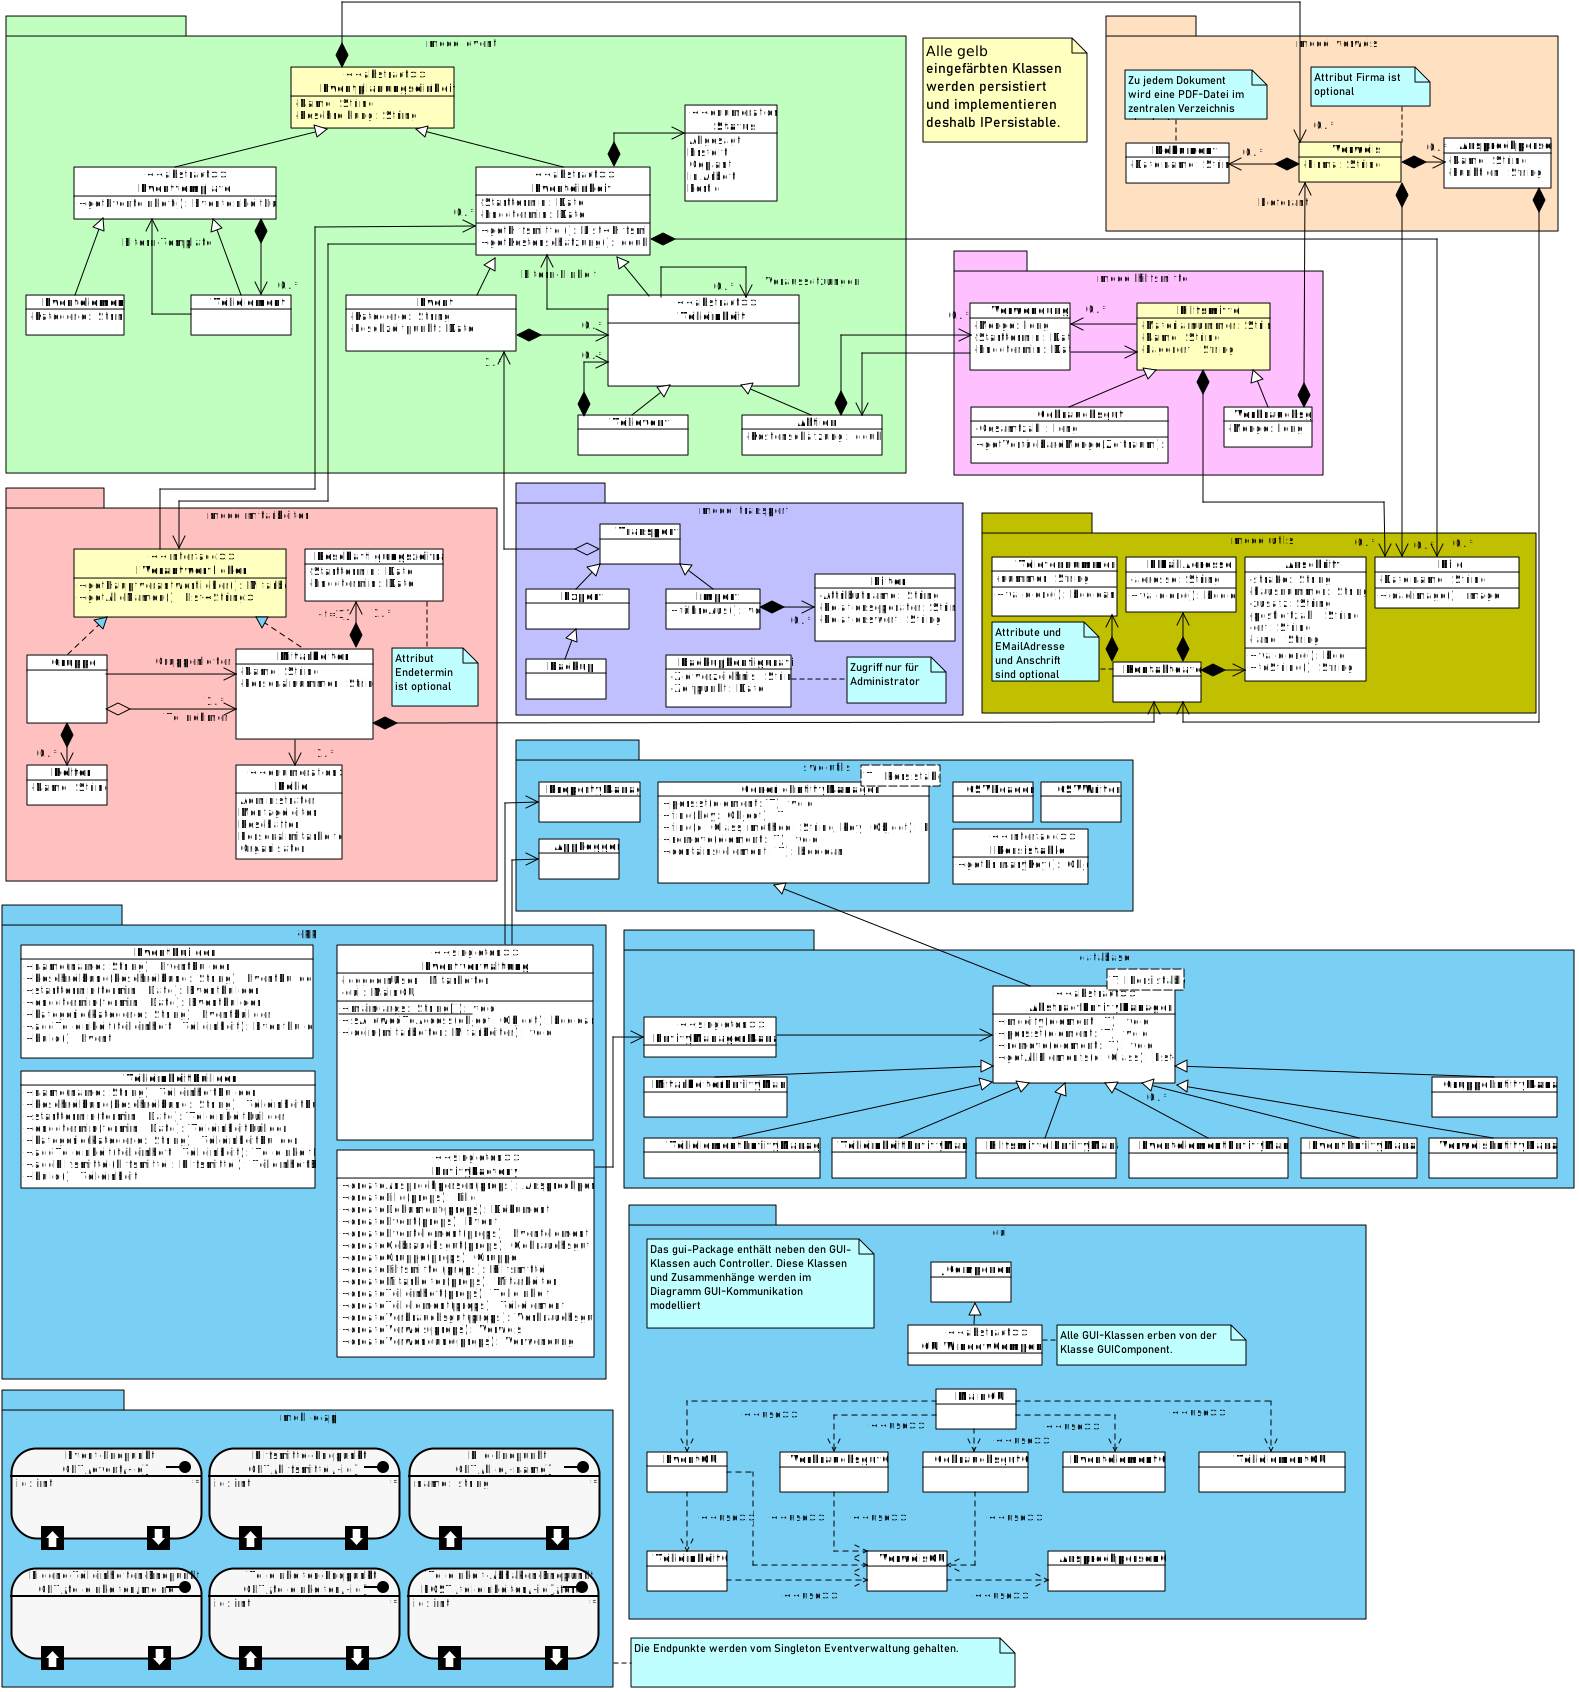
\includegraphics[width=0.98\columnwidth]{Bilder/ekd.pdf}
    \caption{Entwurfsklassendiagramm der Eventplanungssoftware}
\end{figure}

\section{Pakete}

\subsection{model.event}
Dieses Paket enthält alle Klassen aus dem Analyseklassendiagramm, welche Events, Teileinheiten und deren jeweilige Templates betreffen. Da es möglich sein soll, die Events bis zu 14 Tage nach dem Löschen wiederherzustellen, wird ein Event zunächst nur als zu löschend markiert und versteckt. Erst nach 14 Tagen wird es  endgültig aus der Datenbasis gelöscht. Wie man sieht, sind die Klassen Eventplanungseinheit, Eventtemplate sowie Eventplanungseinheit nun abstrakt, da diese nicht instanziiert werden sollen und lediglich der strukturierung der Klassenhierarchie dienen. Ferner sind die Status nun nicht mehr als Unterklassen einer Superklasse \enquote{Status} modelliert, sondern als Enumeration. Die Klasse Teileinheit ist nun ebenfalls abstrakt, da sie nun als Superklasse der Klassen \enquote{Aktion} und \enquote{Teilevent} dient. Diese Unterscheidung ist notwendig, da den Teilevents, welche weitere ihnen untergeordnete Kinderteilevents besitzen, keine Hilfsmittel zugeordnet werden dürfen. Ebenso dürfen den Aktionen, welche Hilfsmittel besitzen dürfen, keine Kinderteileinheiten untergeordnet werden. Darum besitzt nun nur noch die Klasse \enquote{Teilevent} eine Rückassoziation auf die Teileinehit und nur noch die Klasse \enquote{Aktion} eine Assoziation zu \enquote{Verwendung}. Es können jedoch weiterhin beiden Arten von Teilevents weitere Teileinheiten als Voraussetzungen zugeordnet werden.

\subsection{model.verweis}
Dieses Paket enthält neben der Klasse \enquote{Verweis} lediglich \enquote{Dokument} und \enquote{Ansprechperson}, da diese die wesentlichen Bestandteile eines Verweises bilden. Diese konnten vollständig aus dem Analyseklassendiagramm übernommen werden.

\subsection{model.hilfsmittel}
In diesem Paket befinden sich alle Klassen, welche Hilfsmittel sowie deren Zuordnung zu Aktionen betreffen. Die eigentlichen Klassen konnten komplett aus dem Analyseklassendiagramm übernommen werden. Lediglich die Klasse \enquote{Verwendung} besitzt nun nicht mehr eine Assoziation zu der nun abstrakten Klasse \enquote{Teileinheit}, sondern zur Klasse \enquote{Aktion}.

\subsection{model.transport}
Auch die Klassen dieses Paketes, welche den gesamten Datenimport- und export abbilden, konnten vollständig aus dem Analyseklassendiagramm übernommen werden. Um die Übertragung der vorhandenen Eventdaten aus den Excel-Tabellen zu realisieren, wurde keine zusätzliche Funktionalität eingeplant, da diese manuell erfolgen wird.

\subsection{model.mitarbeiter}
Dieses Paket enthält alle Klassen, welche die Verwaltung der Mitarbeiter und deren Zuordnung zu Gruppen betreffen. Hier wurde die Klasse \enquote{Verantwortlicher} in ein Interface umgewandelt, welches von den Klassen \enquote{Gruppe} und \enquote{Mitarbeiter} implementiert wird. Ferner wurden, ähnlich den Status, die Benutzerrollen zu einer Enumeration zusammengefasst, statt sie als einzelne Klassen mit einer Superklasse zu modellieren.

\subsection{model.utils}
In diesem Paket wurden alle Klassen zusammengefasst, welche in mehreren der zuvor beschriebenen Pakete Verwendung finden und darum nicht eindeutig zugeordnet werden konnten. Konkret handelt es sich um die Klassen \enquote{Bild} und \enquote{Kontaktdaten} sowie \enquote{Telefonnummer}, \enquote{EMailAdresse} und \enquote{Anschrift} als Bestandteile der Kontaktdaten.

\subsection{app}
Im Paket \enquote{app} befindet sich zum einen die zentrale Klasse \enquote{Eventverwaltung} mit der Main-Methode zum Starten der Anwendung, welche als Singleton implementiert wird. Sie hält außerdem den \enquote{AppLogger} und den \enquote{PropertyManager} der Anwendung. Ferner befindet sich in diesem Paket das Singleton \enquote{EntityFactory}, eine Fabrikklasse zur Erzeugung von Instanzen derjenigen Klassen, welche in der Datenbasis persistiert werden können. Für die beiden komplexen Klassen \enquote{Event} und \enquote{Teileinheit} existieren in dem Paket außerdem die entsprechenden Builderklassen.

\subsection{database}
Das zentrale Element dieses Paketes ist die abstrakte Klasse \enquote{AbsractEntityManager}, welche von der Klasse \enquote{GenericEntityManager} aus den swe-utils erbt. Der \enquote{AbstractEntityManager} bildet die Superklasse aller konkreten Entity Manager für die zu persistierenden Klassen. Instanziiert und gehalten werden diese durch den \enquote{EntityManagerManager}.

\subsection{gui}
In diesem Paket befinden sich alle Klassen, welche die Benutzeroberfläche betreffen. Die Klassen mit der Endung \enquote{GUI} bilden die Views der Benutzeroberfläche und erben alle von der abstrakten Klasse \enquote{GUIComponent}, welche wiederum von \enquote{JComponent} erben. Die Vererbungspfeile von den Viewklassen zu \enquote{GUIComponent} wurden im Sinne der Übersichtlichkeit nicht dargestellt. Im nachfolgenden Kapitel wird näher auf die Klassen der Benutzeroberfläche eingegangen.

\subsection{swe-utils}
Hier wird lediglich ein Auszug des gesamten Paketes \enquote{swe-utils} dargestellt, nämlich diejenigen Klassen und Interfaces, welche für dieses Projekt verwendet wurden. Dies sind neben den bereits in anderen Paketen erwähnten Klassen, der \enquote{CSVReader} sowie der \enquote{CSVWriter}, welche in den Entity Managern für die Persistierung der Daten verwendet werden. Auch das zu Beginn des Kapitels erwähnte Interface \enquote{IPersistable} stammt aus diesem Paket.

\subsection{mobile-api}
Dieses Paket enthält REST-Endpunkte zum Abfragen von Events, Teileinheiten, Hilfsmitteln und Bildern, außerdem einen separaten Endpunkt zum Abfragen der Teileinheiten, welche einem bestimmten Mitarbeiter zugeordnet sind und schließlich einen Endpunkt zum \enquote{abhaken} abgeschlossener Teileinheiten. Diese bilden die Grundlage der späteren Mobile App in der zweiten Ausbaustufe der Software und werden darum in der jetzigen Phase des Projekts nicht implementiert.

Jeder Endpunkt geht davon aus, dass ein eingeloggter Nutzer die Anfrage stellt und damit in einem Cookie die Session gespeichert ist. Dadurch kann festgestellt werden, welcher Nutzer eingeloggt ist und somit auf welche Objekte zugegriffen werden kann und auf welche nicht.

Die Endpunkte erhalten jeweils Anfrageparameter als Teil der URL und senden Antworten in JSON. Die einzelnen Parameter und Antworten werden im Folgenden näher erläutert, dabei sind die URL-Parameter jeweils in geschweiften Klammern dargestellt. Die Antworten sind schematisch als TypeScript-Objekt angegeben, Referenzen auf andere Elemente haben dabei jeweils den Typen des Primärschlüssels des referenzierten Objektes.
\newpage
\begin{longtable}{l|c|l}
    Endpunkt & Parameter & Antwort \\
    \hline
    GET /event/\{id\} & ID des Events & \begin{lstlisting}[style=json-web-schnittstelle]
{
 id: number,
 name: string,
 beschreibung: string,
 starttermin: Date,
 endetermin: Date,
 verantwortlicher: {
  personalnummer: string,
  name: string
 },
 teilelemente: number[],
 bilder: string[],
 verweise: {
  firma: string?,
  dokumente: File[],
  ansprechpersonen: {
   name: string,
   funktion: string,
   eMailAdresse: string,
   telefonnummer: string,
   anschrift: {
    straße: string,
    hausnummer: string,
    zusatz: string,
    postleitzahl: string,
    ort: string,
    land: string
   }
  }[] 
 }[],
 kategorie: string,
 status: string
}
\end{lstlisting} \\
    \hline
    GET /hilfsmittel/\{id\} & Materialnummer des Hilfsmittels & \begin{lstlisting}[style=json-web-schnittstelle]
{
 materialnummer: string,
 name: string,
 lagerort: string,
 typ: string
}
    \end{lstlisting} \\
    \hline
    GET /bild/\{name\} & Dateiname des Bildes & File \\
    \hline
    GET /teileinheiten/meine & - & \begin{lstlisting}[style=json-web-schnittstelle]
{
    teileinheiten: number[]
}
    \end{lstlisting}\\
    \hline
    GET /teileinheiten/\{id\} & ID der Teileinheit & \begin{lstlisting}[style=json-web-schnittstelle]
{
 id: number,
 name: string,
 beschreibung: string,
 starttermin: Date,
 endetermin: Date,
 verantwortlicher: {
  personalnummer: string,
  name: string
 },
 teilelemente: number[],
 bilder: string[],
 verweise: {
  firma: string?,
  dokumente: File[],
  ansprechpersonen: {
   name: string,
   funktion: string,
   eMailAdresse: string,
   telefonnummer: string,
   anschrift: {
    straße: string,
    hausnummer: string,
    zusatz: string,
    postleitzahl: string,
    ort: string,
    land: string
   }
  }[] 
 }[],
 status: string,
 eltern: number,
 voraussetzungen: number[],
 hilfsmittel: {
  materialnummer: string,
  menge: number
 }[]
}
    \end{lstlisting}\\
    \hline
    POST /teileinheiten/\{id\}/fertig & - & - \\
\end{longtable}

\section{Entwurfsmuster}
Entwurfsmuster sind bewährte wiederverwendbare Vorlagen für die Lösung häufig auftretender Probleme beim Entwurf von Softwaresystemen. Diese Muster haben den Vorteil, dass sie viele bekannte Probleme lösen. In unserer Eventplanungssoftware verwenden wir einige solche Muster, die im Folgenden beschrieben werden.
\subsection{EntityFactory}
Um einzelne Instanzen der Klassen zu erstellen, wird mit der EntityFactory das Muster der EntityFactory umgesetzt. Diese hat eine Methode zum Erstellen eines jeden Objektes und gibt jeweils nach Persitierung im entsprechenden EntityManager eine Instanz des Objektes zurück. Der Übersichtlichkeit wegen wurden die einzelnen Attribute im Diagramm mit \enquote{props} abgekürzt dargestellt. Die EntityFactory ist auch als Singleton modelliert.
\subsection{Singleton}
Im Entwurf sind mehrere Singletons zu finden, dazu gehören die Eventverwaltung, die EntityFactory, der EntityManagerManager und der GUIController. Dadurch soll garantiert werden, dass jeweils nur eine Instanz der Klasse vorhanden ist. Der Sinn dieses Entwurfsmuster ist erkennbar am Beispiel des EntityManagerManagers. Dieser hält eine Instanz des jeweiligen EntityManagers für die spezifische Klasse. Dadurch, dass es immer nur einen EntityManagerManager gibt, ist sichergestellt, dass auch die EntityManager nur einmalig vorhanden sind und somit keine Dateninkonsistenzen auftreten.
\subsection{Builder}
Zum Erstellen der komplexeren Klassen Event und Teileinheit werden Builder bereitgestellt. Damit wird das Objekt Schritt für Schritt erstellt werden und der Zwischenstand stets in dem Builder-Objekt gehalten. Das macht das Erstellen von Event- und Teileinheitobjekten deutlich ergonomischer.
\subsection{Kompositum}
Um die Teil-Ganzes-Hierarchie von Teileinheit zu Unterteileinheiten darzustellen, wird das Kompositum-Muster verwendet. Es wird die Baumstruktur von Teileinheiten, welche Unterteileinheiten besitzen können, abgebildet. Dafür gibt es die Klasse Teileinheit, von welcher Aktion und Teilevent erben. 
\subsection{Beobachter}
Die Beobachter wurden im Entwurf passiv implementiert, daher werden diese lediglich benachrichtigt, wenn Änderungen aufgetreten sind. Die Beobachter fragen nicht aktiv den Zustand des konkreten Subjektes an, da sie das konkrete Subjekt nicht kennen. Dieses ermöglicht eine hohe Abstraktionsmöglichkeit und Wiederverwendbarkeit der einzelnen Komponenten.
\subsection{EntityManager}
Es wurde sich dafür entschieden, konkrete EntityManager pro Klasse zu implementieren, jedoch werden Aktionen und Teilevents sowie Gebrauchsgüter und Verbrauchsgüter jeweils zusammen im TeileinheitEntityManager und HilfsmittelEntityManager verwaltet. Diese Implementierung hat den großen Vorteil, dass die Serialisierung zum Schreiben in CSV-Dateien für jede Klasse einzeln geschrieben werden kann und damit somit weniger Einschränkungen dabei bestehen. Alle konkreten EntityManager erben vom AbstractEntityManager, welcher vom GenericEntityManager aus den swe-utils erbt. Dadurch ist eine gemeinsame Schnittstelle aller EntityManager und trotzdem die Konkretisierung in jeder einzelnen Implementierung vorhanden.
